\documentclass[a4paper]{uebungsblatt}
%\blattuntertitel{Untertitel des Blatts}
\begin{document}

\begin{aufgabe}[a]
	\teilaufgabe
	Mit Hilfe von Abbildung \ref{abb:kdf1} und NIST SP800-108 erkl\"art sich die Funktionsweise dieser KDF\footnote{Key Derivation Function} wie folgt: 
	\begin{figure}[H]
		\centering
		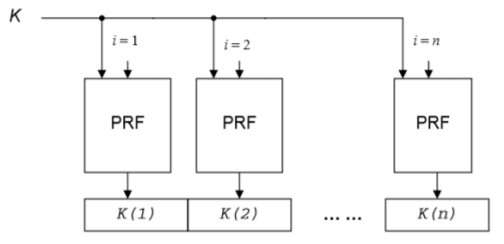
\includegraphics[scale=0.6]{kdf1.png}
		\caption{Aus dem \"Ubungsblatt}\label{abb:kdf1}
	\end{figure}
	Vom Eingangsschl\"ussel $ K $ mit der L\"ange $ n $ wird ein Ausgangsschl\"ussel $ K(1),K(2),\ldots,K(n) $ abgeleitet. Dazu wird die $ i $-te Stelle des Eingangsschl\"ussel durch eine definierte PRF\footnote{Pseudo-Random Function} auf $ K(i) $ transformiert. Wenn $ K(i) $ l\"anger ist als die $ i $-te Stelle, dann wird der Eingangsschl\"ussel auf den Ausgangsschl\"ussel \enquote{expandiert}.
	
	\teilaufgabe
	In Kapitel 4 des Standards werden als geeignete Primitive f\"r die PRF MACs\footnote{Message Authentication Code} genannt: Kryptographische Algorihmen, die mit symmetrischen Schl\"usseln arbeiten. Sie k\"onnen verschieden lange Inputwerte auf immer gleich lange Ausgangswerte transformieren. Untergruppe davon sind HMAC und CMAC.\\
	Zus\"ätzlich eignen sich Verkettete Verschl\"usselungen / Blockchiffre als Kandidaten f\"ur die PRF, bekannt aus KVA 1: CBC \footnote{Cipher Block Chaining Mode}, OFB \footnote{Output Feedback Mode}, CFB \footnote{Cipher Feedback Mode} und CTR \footnote{Counter Mode}. 
	
	\teilaufgabe
	Die im Standard beschriebenen KDFs erinnern an bekannte Konstruktionen.\\
	Die erste KDF, siehe Abbildung \ref{abb:kdf2}, ist eine Hashkonstruktion, weil unterschiedlicher Input in Bl\"ocke gleicher L\"ange ausgegeben wird. Au{\ss}erdem wird die Ausgabe nicht weiter in den folgenden Schritten ber\"ucksichtigt. Die zweite KDF in Abbildung \ref{abb:kdf3} hat eben diese Verkettung zwischen vorherigem Ausgabeblock und n\"achstem Eingabeblock, sie erinnert also an eine CBC-Konstruktion.\\
	Die dritte und letzte KDF in Abbildung \ref{abb:kdf4} ist stellt eine Addition der beiden vorherigen dar: Der obere Teil ist ein CBC, dessen schrittweise Ausgabe nochmal gehasht wird.
	
	\begin{figure}[H]
		\centering
		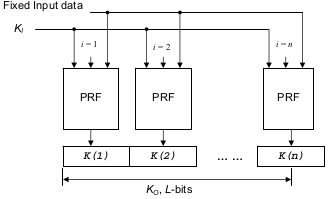
\includegraphics[scale=0.6]{kdf2.png}
		\caption{Aus dem Standard (Figure 1): \enquote{KDF in Counter-Mode}}\label{abb:kdf2}
	\end{figure}
		
	\begin{figure}[H]
		\centering
		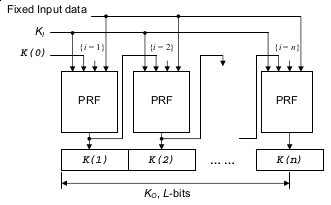
\includegraphics[scale=0.6]{kdf3.png}
		\caption{Aus dem Standard (Figure 3): \enquote{KDF in Feedback Mode}}\label{abb:kdf3}
	\end{figure}
	
	\begin{figure}[H]
		\centering
		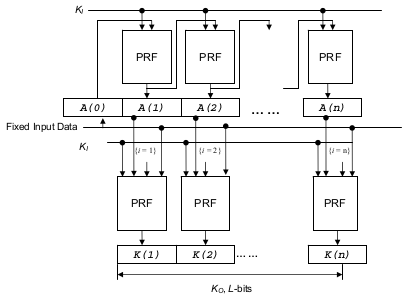
\includegraphics[scale=0.6]{kdf4.png}
		\caption{Aus dem Standard (Figure 4): \enquote{KDF in Double-Pipeline Iteration Mode}}\label{abb:kdf4}
	\end{figure}

	\teilaufgabe
	Nach der Betrachtung der Konstruktion ist klar, dass der Eingangsschl\"ussel so zuf\"allig sein muss, dass er mit hoher Wahrscheinlichkeit einmalig ist. Diese Einmaligkeit ist nicht bei allen Passw\"ortern gegeben. Ein Angreifer macht sich den beschr\"ankten Passwortraum (im Vergleich zum unbeschr\"ankten zuf\"alligen Schl\"usselraum) zur Nutze und berechnet f\"ur alle m\"oglichen Eingaben im Passwortraum die ausgegebenen Werte. Abschlie{\ss}end vergleicht er die den anzugreifenden Ausgabewert mit seinen Berechneten und kann bei Gleichheit auf den Eingabewert schlie{\ss}en.

\end{aufgabe}

\end{document}

